%\documentclass[conference,final]{IEEEtran}
%\documentclass{acm_proc_article-sp}

% \documentclass{sig-alternate}
\documentclass{sig-alt-release2}

\usepackage[numbers, sort, compress]{natbib}
\usepackage{graphicx}
\usepackage{amsmath}
\usepackage{amssymb}
\usepackage{color}
\usepackage{ifpdf}

\usepackage{dcolumn}
\usepackage{float}
\usepackage[utf8]{inputenc}
\usepackage{multirow}
\usepackage{rotating}

\usepackage[tight]{subfigure}



%\usepackage[numbers, sort, compress]{natbib}
%\usepackage{latex8}
%\usepackage{float}
%\usepackage{times}    
\usepackage{url}
\usepackage{listings}   
\usepackage{paralist}    
\usepackage{wrapfig}    
%\usepackage[small,it]{caption}
\usepackage{multirow}
\usepackage{ifpdf}
%\usepackage{srcltx}
%\usepackage{subfigure}
\usepackage{xspace}
\usepackage{keyval}  
\usepackage{color}

\definecolor{listinggray}{gray}{0.95}
\definecolor{darkgray}{gray}{0.7}
\definecolor{commentgreen}{rgb}{0, 0.4, 0}
\definecolor{darkblue}{rgb}{0, 0, 0.4}
\definecolor{middleblue}{rgb}{0, 0, 0.7}
\definecolor{darkred}{rgb}{0.4, 0, 0}
\definecolor{brown}{rgb}{0.5, 0.5, 0}

\usepackage[normalem]{ulem}
\makeatletter
\def\cyanuwave{\bgroup \markoverwith{\lower3.5\p@\hbox{\sixly \textcolor{cyan}{\char58}}}\ULon}
\def\reduwave{\bgroup \markoverwith{\lower3.5\p@\hbox{\sixly \textcolor{red}{\char58}}}\ULon}
\def\blueuwave{\bgroup \markoverwith{\lower3.5\p@\hbox{\sixly \textcolor{blue}{\char58}}}\ULon}
\font\sixly=lasy6 % does not re-load if already loaded, so no memory problem.
\makeatother


\begin{document}

\conferenceinfo{HPDC'12,} {June 18--22, 2012, Delft, The Netherlands.} 
\CopyrightYear{2012} 
\crdata{978-1-4503-0805-2/12/06} 
\clubpenalty=10000 
\widowpenalty = 10000

%!TEX root = sc12/pstar-sc2012-ieee.tex
\newif\ifdraft
%\drafttrue
\ifdraft
\newcommand{\onote}[1]{ {\textcolor{cyan} { (***Ole: #1) }}}
\newcommand{\terminology}[1]{ {\textcolor{red} {(Terminology used: \textbf{#1}) }}}
\newcommand{\owave}[1]{ {\cyanuwave{#1}}}
\newcommand{\jwave}[1]{ {\reduwave{#1}}}
\newcommand{\alwave}[1]{ {\blueuwave{#1}}}
\newcommand{\jhanote}[1]{ {\textcolor{red} { ***shantenu: #1 }}}
\newcommand{\alnote}[1]{ {\textcolor{blue} { ***andreL: #1 }}}
\newcommand{\amnote}[1]{ {\textcolor{blue} { ***andreM: #1 }}}
\newcommand{\smnote}[1]{ {\textcolor{brown} { ***sharath: #1 }}}
\newcommand{\msnote}[1]{ {\textcolor{cyan} { ***mark: #1 }}}
\newcommand{\note}[1]{ {\textcolor{magenta} { ***Note: #1 }}}
\else
\newcommand{\onote}[1]{}
\newcommand{\terminology}[1]{}
\newcommand{\owave}[1]{#1}
\newcommand{\jwave}[1]{#1}
\newcommand{\alnote}[1]{}
\newcommand{\amnote}[1]{}
\newcommand{\athotanote}[1]{}
\newcommand{\smnote}[1]{}
\newcommand{\jhanote}[1]{}
\newcommand{\msnote}[1]{}
\newcommand{\note}[1]{}
\fi

\newcommand{\pilot}{Pilot\xspace}
\newcommand{\pilots}{Pilots\xspace}
\newcommand{\pilotjob}{Pilot-Job\xspace}
\newcommand{\pilotjobs}{Pilot-Jobs\xspace}
\newcommand{\computeunit}{Compute Unit\xspace}
\newcommand{\computeunits}{Compute Units\xspace}
\newcommand{\cu}{CU\xspace}
\newcommand{\cus}{CUs\xspace}
\newcommand{\cs}{Compute Service\xspace}
\newcommand{\css}{Compute Services\xspace}
\newcommand{\pcs}{Pilot Compute Service\xspace}
\newcommand{\dataunit}{Data Unit\xspace}
\newcommand{\dataunits}{Data Unit\xspace}
\newcommand{\du}{DU\xspace}
\newcommand{\dus}{DUs\xspace}
\newcommand{\pilotdata}{Pilot-Data\xspace}
\newcommand{\pd}{PD\xspace}
\newcommand{\pds}{Pilot Data Service\xspace}
\newcommand{\pdss}{Pilot Data Services\xspace}
\newcommand{\su}{SU\xspace}
\newcommand{\sus}{SUs\xspace}
\newcommand{\schedulableunit}{Schedulable Unit\xspace}
\newcommand{\schedulableunits}{Schedulable Units\xspace}
\newcommand{\cc}{c\&c\xspace}
\newcommand{\CC}{C\&C\xspace}

\lstdefinestyle{myListing}{
  frame=single,   
  backgroundcolor=\color{listinggray},  
  %float=t,
  language=C,       
  basicstyle=\ttfamily \footnotesize,
  breakautoindent=true,
  breaklines=true
  tabsize=2,
  captionpos=b,  
  aboveskip=0em,
  belowskip=-2em,
  %numbers=left, 
  %numberstyle=\tiny
}      

\lstdefinestyle{myPythonListing}{
  frame=single,   
  backgroundcolor=\color{listinggray},  
  %float=t,
  language=Python,       
  basicstyle=\ttfamily \footnotesize,
  breakautoindent=true,
  breaklines=true
  tabsize=2,
  captionpos=b,  
  %numbers=left, 
  %numberstyle=\tiny
}

\newcommand{\up}{\vspace*{-1em}}
\newcommand{\upp}{\vspace*{-0.5em}}
\newcommand{\numrep}{8 }
\newcommand{\samplenum}{4 }
\newcommand{\tmax}{$T_{max}$ }
\newcommand{\tc}{$T_{C}$ }
\newcommand{\tcnsp}{$T_{C}$}
\newcommand{\bj}{BigJob}

%  \setlength{\parskip}{0.05ex} % 1ex plus 0.5ex minus 0.2ex}
%  \setlength{\parsep}{0pt}
%  %\setlength{\headsep}{0pt}
%  \setlength{\topskip}{0pt}
%  \setlength{\topmargin}{0pt}
%  %\setlength{\topsep}{0pt}
%  \setlength{\partopsep}{0pt}

% This is now the recommended way for checking for PDFLaTeX:


\ifpdf
\DeclareGraphicsExtensions{.pdf, .jpg, .tif}
\else
\DeclareGraphicsExtensions{.eps, .jpg}
\fi

\tolerance=1000
\hyphenpenalty=10




\title{Towards a Common Model for Pilot-Jobs\up}

\numberofauthors{2}
\author{
\alignauthor Andre Luckow, Ole Weidner, \\Andre Merzky, Sharath Maddineni\\
       \affaddr{Center for Computation and Technology}\\
       \affaddr{Louisiana State University}\\
       %\affaddr{216 Johnston}\\
       \affaddr{Baton Rouge, LA} \\
       \email{\{aluckow, oweidern, amerzky, smaddini\}@cct.lsu.edu}
\and
\alignauthor Mark Santcroos\\
       \affaddr{Bioinformatics Laboratory}\\
       \affaddr{Academic Medical Center}\\
       \affaddr{University of Amsterdam}\\
       % \affaddr{Meibergdreef 9}\\
       \affaddr{Amsterdam, The Netherlands}
       \email{m.a.santcroos@amc.uva.nl}
\and
\alignauthor Shantenu Jha\footnote{Contact Author}\\
      \affaddr{CAC/ECE}\\
     \affaddr{Rutgers University}\\
      % \affaddr{94 Brett Road}\\
      \affaddr{Piscataway, NJ}
     \email{shantenu.jha@rutgers.edu}
}

\date{}

\maketitle

\let\thefootnote\relax\footnotetext{$^{*}$contact author}

\vspace{-2cm}
\begin{abstract} 
  \pilotjobs (PJ) have become one of the most successful abstractions in
  distributed computing. In spite of extensive uptake, there does not
  exist a well defined, unifying conceptual model of \pilotjobs, which
  can be used to define, compare and contrast PJ
  implementations. This presents a barrier to extensibility and
  interoperability. This paper is an attempt to, (i) provide a minimal
  but complete model (P*) of \pilotjobs, (ii) establish the generality
  of the P* Model by mapping various well-known \pilotjob
  frameworks such as Condor and DIANE to P*, (iii) demonstrate the
  interoperable and concurrent usage of {\it distinct} pilot-job
  frameworks on different production distributed cyberinfrastructures
  via the use of an extensible API for the P* Model (Pilot-API).
\end{abstract}

% derive an interoperable and extensible API for the P* Model
% (Pilot-API), and (iv) validate the implementation of the Pilot-API by
% concurrently using multiple {\it distinct} pilot-job frameworks on
% distinct production distributed cyberinfrastructures.  \jhanote{We
%   should be careful as to whether to say if this paper addresss (iii)?
%   We don't discuss Pilot-API and we don't validate using the
%   implementation using concurrent pilot-job frameworks?  Maybe
%   rephrase (iii) and (iv)?}

\category{D.2.10}{Software Design}{Methodologies}
\keywords{Distributed Systems, Interoperability, Abstractions}


\upp
\section{Introduction and Overview} 

Distributed cyber/e-infrastructure is by definition comprised of a set
of resources that is fluctuating -- growing, shrinking, changing in
load and capability (in contrast to a static resource utilization
model of traditional cluster computing systems).  The
ability to utilize a dynamic resource pool is thus an important
attribute of any application that needs to utilize distributed
cyberinfrastructure (DCI) efficiently. \pilotjobs (PJ) provide an
effective abstraction for dynamic execution and resource utilization
in a distributed context. As a consequence of providing a simple
approach for decoupling workload management and resource
assignment/scheduling, \pilotjobs have been one of the most successful
abstractions in distributed computing.  Not surprisingly, there are
multiple, distinct and incompatible implementations of
\pilotjobs. Often, these implementations are coupled to the
infrastructure they were designed for.

Our objective is to provide a minimal, but complete model of
\pilotjobs: The P* Model provides a conceptual basis to compare and
contrast different PJ frameworks.  We perform experiments
demonstrating interoperability across middleware, platform and
different PJ frameworks, and to establish the effectiveness of the
Pilot-API.


\section{The P* Model of Pilot-\\Abstractions}
\label{sec:pilot-model}

The P* model is derived from an analysis of many PJ implementations;
based upon this analysis, we present the common {\it elements} of the P*
Model, followed by a description of the overall functioning of a PJ framework. 
The P* Model defines the following elements:

\begin{figure}[t]
	\upp\upp
    \centering
    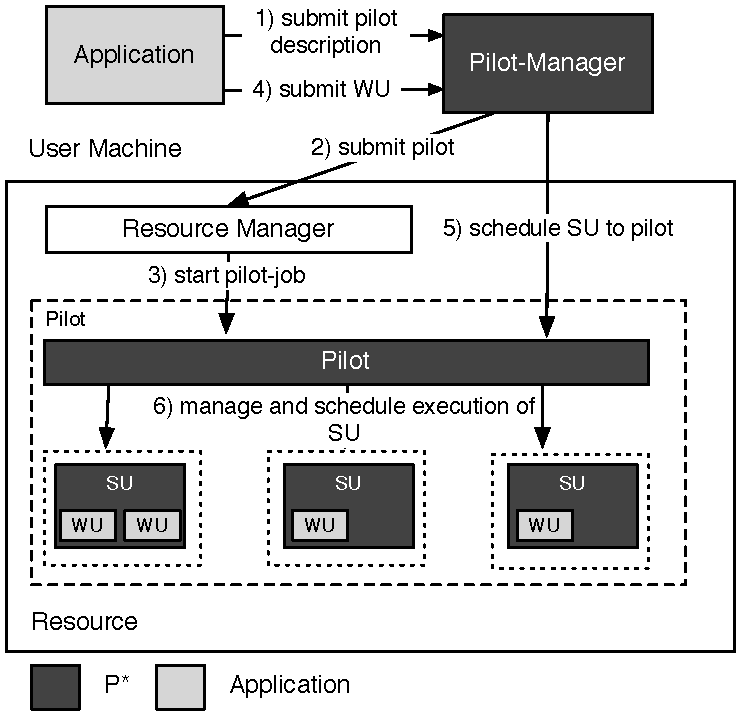
\includegraphics[width=0.37\textwidth]{figures/pstar_model_single.pdf}
    \caption{ \textbf{P* Model: Elements and
        Interactions:} The manager has two functions: it manages 1)
      Pilots (step 1-3) and 2) the execution of \cus. After a \cu is
      submitted to the manager, it transitions to an \su, which is
      scheduled to a \pilot by the PM.}
	\upp\upp
    \label{fig:figures_pstar}
\end{figure}


\noindent$\bullet$ \textbf{\pilot (Pilot-Compute):} The \pilot is the
  entity that actually gets submitted and scheduled on a resource.
  The PJ provides application (user)
  level control and management of the set of allocated resources.



\noindent$\bullet$ \textbf{\computeunit  (\cu):} A \cu  encapsulates a 
  self-contained piece of work (a task) specified by the application that is
  submitted to the \pilotjob framework. There is no intrinsic notion
  of resource associated with a \cu.

\noindent$\bullet$ \textbf{Scheduling Unit (SU):} SUs are the units of 
  scheduling, internal to the P* Model, i.e., it is not known by or
  visible to an application. Once a \cu is
  under the control of the \pilotjob framework, it is assigned
  to an SU.


\noindent$\bullet$ \textbf{Pilot-Manager (PM):} The PM is responsible for (i)
  orchestrating the interaction between the \pilots as well as the
  different components of the P* Model (\cus, \sus) and (ii) decisions
  related to internal resource assignment (once resources have been
  acquired by the \pilotjob).  For example, an SU can consists of one
  or more \cus. %Further, \cus and \sus can be combined and aggregated;
  The PM determines how to group them and when \sus are scheduled and
  executed on a resource via the \pilot.


Figure~\ref{fig:figures_pstar} illustrates the interactions between the
elements of the P* Model. First, the application specifies the capabilities of
the resources required using a \pilotjob description (step 1). The PM then
submits the necessary number of \pilots to fulfill the resource requirements
of the application (step~2). Each \pilot is queued at the resource manager,
which is responsible for starting it (step~3). The application can
submit \cus to the PM at any time (step~4). A submitted \cu \ becomes an SU,
i.\,e.\ the PM is now in control of it. In the simplest case one \cu  corresponds to one SU. 



\begin{table}[t]
  \upp
 \footnotesize
 \centering
 \begin{tabular}{|p{1.5cm}|p{1.5cm}|p{1.5cm}|p{2.5cm}|}
  \hline
  \textbf{P* Element}    &\textbf{BigJob} &\textbf{DIANE} &\textbf{Condor-G/Glide-in}  \\\hline
  Pilot-Manager          &BigJob Manager  & RunMaster     & condor\_master\newline 
                                                            condor\_collector\newline 
                                                            condor\_negotiator\newline 
                                                            condor\_schedd                \\\hline
  \pilot                 &BigJob Agent    & Worker Agent  &condor\_master\newline
                                                           condor\_startd                 \\\hline
  CU   &Task            &Task           &Job                            \\\hline
  SU &Sub-Job         &Task           &Job                            \\\hline
% Dynamic Resources &no/yes &yes (AgentFactories)\\
% \hline
 \end{tabular}
 \caption{\textbf{Mapping P* elements and PJ Frameworks:} While each
   PJ framework maintains its own vocabulary, each of the P* elements
   can be mapped to one (or more) components of the different
   frameworks. \upp \upp \upp}
 \label{table:bigjob-saga-diane}
\end{table}


As shown in table~\ref{table:bigjob-saga-diane}, the above elements
can be mapped to specific entities in different \pilotjobs framework,
e.\,g.\ BigJob~\cite{saga_bigjob_condor_cloud_short},
Condor~\cite{condor-g-short} and DIANE~\cite{Moscicki:908910}. While
most of these frameworks share many properties, they often differ in
their implementation (e.\,g.\ of the communication mechanism) and
usage modalities. 
The aim of the Pilot-API~\cite{pilot_api} is to provide an abstract,
unified interface to PJ frameworks that adhere to the P* Model.
Figure~\ref{fig:perf_perf-bfast-bj} shows how the Pilot-API enables
the user to run applications interoperably on different production and
research infrastructures. For this purpose we investigate the
performance of BFAST, a genome sequencing
application. BFAST is very I/O sensitive -- we observed for example,
an I/O bottleneck if many BFAST CUs are run on the same shared file
system. 
The Pilot-API enables applications to scale to different
infrastructures in such cases.

 
\begin{figure}[t]
	\upp
\centering
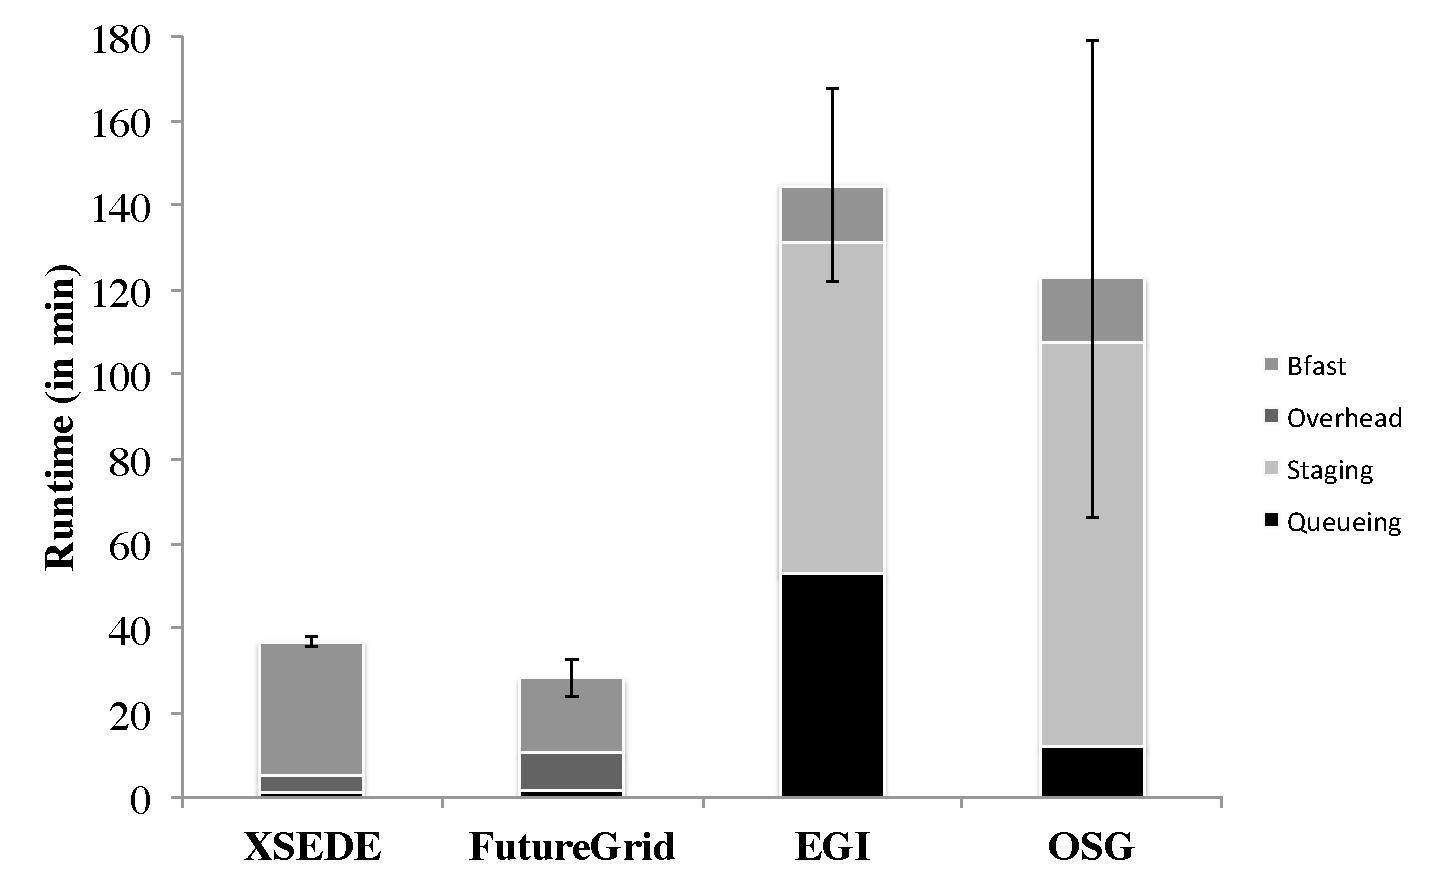
\includegraphics[width=0.4\textwidth]{perf/interop/128-bfast-egi-fg-xsede-osg.pdf}
\caption{\textbf{PJ Framework Performance on XSEDE, FutureGrid, EGI and 
  OSG:} Running 128 BFAST match tasks on 128 cores. The longer runtimes on EGI 
  and OSG are mainly caused by  longer queuing times and the necessity to   stage all input files. }\upp\upp\upp
  \label{fig:perf_perf-bfast-bj}
\end{figure}


\section{Discussion and Future Work} 
\label{sec:discussion-future-work}

Although a variety of PJ frameworks have emerged, which are, for the
most parts, functionally equivalent, it is often impossible to use
them interoperably or even just to compare them. The primary
contribution of this work is the development of the P* Model, the
usage of the P* elements to describe and characterize PJ frameworks
such as DIANE and Condor-G/Glide-in.  We demonstrated the practical
relevance of this work by using different PJ frameworks via a unified
API, and enabling applications to scale across different
infrastructures and utilize performance advantages.

Pilot-abstractions provide significant future research \& development
opportunities, especially in their use for data-intensive
applications.
% While Pilot-Jobs efficiently support late-binding of\computeunits and resources, 
The management, placement and scheduling of data in distributed
systems remains a challenge due to various reasons: (i) the placement
of data is often decoupled from the placement of Compute Units and
Pilots, i.\,e.\ the application must often manually stage in and out
its data using simple scripts; (ii) heterogeneity, e.\,g.\ with
respect to storage, filesystem types and paths, often prohibits late
binding decisions; (iii) absence of capabilities that allow
applications to specify their data dependencies on an abstract,
logical level (rather than on file basis) are not available; (iv) due
to lack of a common treatment for compute and data, optimizations of
data/compute placements are often not possible. In addition,
applications must cope with various other challenging, data-related
issues, e.\,g.\ varying data sources (such as sensors and/or other
application components), fluctuating data rates, transfer failures,
optimizations for different queries, data-/compute co-location
etc. While these issues can be handled in an application-specific
manner, the use of general-purpose, infrastructure independent
capabilities, such as a common \pilot-based abstraction for compute
and data presents several advantages. This motivates an abstraction
for data, that is analogous to Pilot-Jobs, that we refer to as
\emph{\pilotdata (PD)}.



\bibliographystyle{IEEEtran}
\bibliography{pilotjob,saga,saga-related}


% \bibliography{pstar-hpdc2012}

\end{document}
